% THIS IS SIGPROC-SP.TEX - VERSION 3.1
% WORKS WITH V3.2SP OF ACM_PROC_ARTICLE-SP.CLS
% APRIL 2009
%
% It is an example file showing how to use the 'acm_proc_article-sp.cls' V3.2SP
% LaTeX2e document class file for Conference Proceedings submissions.
% ----------------------------------------------------------------------------------------------------------------
% This .tex file (and associated .cls V3.2SP) *DOES NOT* produce:
%       1) The Permission Statement
%       2) The Conference (location) Info information
%       3) The Copyright Line with ACM data
%       4) Page numbering
% ---------------------------------------------------------------------------------------------------------------
% It is an example which *does* use the .bib file (from which the .bbl file
% is produced).
% REMEMBER HOWEVER: After having produced the .bbl file,
% and prior to final submission,
% you need to 'insert'  your .bbl file into your source .tex file so as to provide
% ONE 'self-contained' source file.
%
% Questions regarding SIGS should be sent to
% Adrienne Griscti ---> griscti@acm.org
%
% Questions/suggestions regarding the guidelines, .tex and .cls files, etc. to
% Gerald Murray ---> murray@hq.acm.org
%
% For tracking purposes - this is V3.1SP - APRIL 2009

\documentclass{acm_proc_article-sp}

\begin{document}



\title{Catchy Part: Surveying Users' Perceptions of Threats for Wearable Devices}
%\titlenote{(Does NOT produce the permission block, copyright information nor page numbering). For use with ACM\_PROC\_ARTICLE-SP.CLS. Supported by ACM.}}

%\subtitle{[Extended Abstract]
%\titlenote{Note
%\textit{Note \LaTeX$2_\epsilon$\ and BibTeX} at \texttt{www.website.com}}}


\numberofauthors{3} 

\author{
% 1st. author
\alignauthor
Linda N. Lee\\
       \affaddr{UC Berkeley}\\
       \email{lnl@berkeley.edu}
% 2nd. author
\alignauthor
Serge Egelman\\
       \affaddr{UC Berkeley}\\
       \affaddr{ICSI}\\
       \email{serge@cs.berkeley.edu}
% 3rd. author
\alignauthor David Wagner\\
       \affaddr{UC Berkeley}\\
       \email{daw@cs.berkeley.edu}
}

\maketitle



\begin{abstract}
Hello world.
\end{abstract}

% A category with the (minimum) three required fields
\category{look it up}{keyword1}{keyword2}{keyword3}
%A category including the fourth, optional field follows...
%\category{D.2.8}{Software Engineering}{Metrics}[complexity measures, performance measures]

\terms{term1} {term2} {term3}

\keywords{Privacy, User Studies, Ubiquitous Computing,Internet of Things} % NOT required for Proceedings

%%%%%%%%%%%%%%%%%%%
%%%         PAPER BODY         %%%
%%%%%%%%%%%%%%%%%%%

\section{Introduction}
Basically a longer version of the abstract, plus some additional motivational things thrown in here. 

2014 is year of wearables \cite{Forbes}. A survey consisting of 3,956 respondents who are either current users or non-users with high interest in wearables \cite{Neilsen} says that most popular devices (61\%), followed by smart watches (45\%) and mHealth (mobile health) devices (17\%). It is estimated that ~15\% use it in daily life \cite{Nilsen}\cite{WearableStatNews}.

End this section with an explicit list of contributions made by this paper.

%%%%%%%%%%%%%%%%%%%

\section{Related Work}
In this paper, we explore user perceptions of security threats for wearable devices. In this section, we discuss related works which explore threats for smartphones and wearable devices, discuss emerging challenges related to ubiquitous computing, and study user perceptions of threats and technologies. 

\subsection{Privacy for Smartphones and Wearables}
(REDO) Mention Adrienne's work here, and other cool smartphone studies of any sort. Be sure to go cite a fair number of them. Related work section is the part where it looks like I know stuff. 

Mention any other privacy studies for wearables (like the ones you can find at Ubicomp, CHI, or SOUPS), and give them a nod. Also highlight how my study is different from previous studies. 

\subsection{Ubiquitous Computing}
(REDO) As technology becomes more and more ubiquitous, more sensors will record more things about more people more of the time. There are an endless amount of unique situations which can negatively impact a person's privacy or security. There is a clear need to better communicate these risks to people (cite webcam paper and other papers here?), but there are too many things to warn people about. Therefore, we need to know what are the most threatening and also most relevant situations to inform the users about, since we can't bug them all the time about everything. 

\subsection{User Perception}
(REDO) In this paper, we investigate one of the two important questions--what are the most relevant situations to people. We do this firstly because people are really bad at knowing the likelihood of something, especially a threat with respect to security or privacy, is going to happen (sources here). And while the most damaging situations should also be addressed, this is not yet possible since these technologies haven't been adopted and the damage hasn't happened, so we don't know yet. Additionally, since the number one concern that people had with these devices was privacy (can I say result here? I guess I already did in abstract), we need to know what people consider private, which is more nuanced and requires a user study like this survey. 

%%%%%%%%%%%%%%%%%%%

\section{Survey}
The survey design process consisted of synthesizing a relevant and comprehensive set of questions, validating the relevance, clarity, and completeness of the questions, and concluded with finalizing distribution logistics. Details on the synthesis, validation, methodology, and data are below.

\subsection{Threat Landscape Investigation} 
(REDO) To generate the list of possible scenarios which can happen with a wearable device, we did three things. Firstly, we looked at the most popular list of wearable technologies (including the Fitbit fitness tracker, Pebble smartwatch, and Glass wearable computing device) and their sensors and capabilities. Secondly, we looked at past research in mobile devices and current wearable device considerations. Thirdly, we finished off brainstorming possible things yet to come by looking at vision videos for wearables, and the news for possible concerns. 

Motivate the fact that this is important here! Mention ubiquitious computing, preventing security threats, etc. 

\subsection{Calibrating with Existing Works}
(REDO) We used the same format as Adrienne's paper so that we can compare our results to the ones that she got in her study for mobile devices. Mobile devices threats are well studied and the closest well-researched thing to wearable device threats. 

We used a prompt similar to Fischoff's study so that we could compare our results to the ones that he got in his study, and to put more of the new technologies onto the risk/benefit map. This way, we can have a sense of the risk and benefit with respect to well-studied and more familiar technologies. 

\subsection{Validation}
(REDO) We conducted a focus group to look over the list, brainstorm more scenarios, and clarify any scenarios which were unclear (we also used this time to time the survey and make sure the formatting was clear. 

\subsection{Methodology}
We recruited 2,250 participants August 7th-13th 2014 via Amazon's Mechanical Turk. We restricted participants to those over 18 years old. No other restrictions on participation were applier. We asked questions regarding participants' perceptions of various situations which might occur when wearing a wearable device, and about the risks and benefits of new technologies.
 
 %%%%%%%%%%%%%%%%%%%
 
\section{Questions}
The survey consisted of questions regarding concerns with respect to a factious wearable device called the Cubetastic3000 (this was done to prevent any biases in answers from participants with respect to specific companies), smartphone concerns, risk and benefit assessment of technologies, and exit questions. Details on the question ordering, question formatting, and sample questions are below. The full survey can be found at <LINK HERE>. 

\subsection{Format}
In total, the survey consisted of 367 unique questions, with each participant answering 27 questions. Out of the 27 seen by the participant, 10 of the questions are randomly selected from a particular set of questions (see below).   \\[-.8cm]

\begin{itemize} \itemsep1pt \parskip0pt \parsep0pt
\item 2 comprehension questions 
\item 6/305 questions about various scenarios 
\item 2/5 questions about smartphone scenarios 
\item 1/20 benefit questions 
\item 1/20 risk questions (same technology) 
\item 4 demographics
\item 1 open-ended question 
\item 10 questions of IUIPC \\[-.8cm]
\end{itemize}

To mitigate any biases, we randomized the order in which users saw groups of questions. That is; the participant has an equal chance of seeing questions related to threat perceptions or questions related to risk and benefit assessment of technologies. Additionally, each question in the sections about various scenarios, questions about smartphone scenarios, and IUIPC questions were randomly selected. A participant was also equally likely to see the risk or benefit questions first when they got to the section pertaining to risk and benefit assessment of technologies. (Ugh this is bad, re-write later)

\subsubsection{Threat Perceptions}
Format of question explanation, list the edge case questions here. Show an example of the question. 

\subsubsection{Technology Perceptions}
Format of the question explanation, list the technologies here (is this too many?). Show an example of the question. 

\subsubsection{User Concerns}
This is an open-ended question. Show the question here. Say that the participants had as much space as they wanted, although they were shown a line. 

\subsubsection{Additional Questions}
demographics and IUIPC, explain why I used IUIPC instead of the Westin, just one or two sentences will do. 

%%%%%%%%%%%%%%%%%%%

\section{Results}
After removing X incomplete responses, our sample consisted of Y participants. Of these X, A\% were male, with a median age of B. Two researchers independently coded 1,785 open-ended responses, discussed any disagreements, and resolved them so that the final codings reflect unanimous agreement. 

\subsection{Factors in Upsetting Users}
We found that the data type and data recipient, respectively, are the most significant predictors of how upsetting or threatening a situation is perceived by a user. On the other hand, the device type does not significantly impact how users perceive a situation.

\subsubsection{Data Type}
blah blah here. 

%For all recipients \\[-.8cm]
%
%\begin{enumerate} \itemsep1pt \parskip0pt \parsep0pt
%  %\setcounter{enumi}{0}
%  \item a video of you unclothed
%  \item bank account information
%  \item social security number
%  \item video of you entering in your PIN
%  \item a photo of you unclothed
%  \item a photo of you that is incriminating or embarrassing
%  \item username and password for websites
%  \item credit card information
%  \item a video of you that is incriminating or embarassing
%  \item a photo you at home taken randomly by an inward-facing camera \\[-.8cm]
%\end{enumerate}
%
%\begin{enumerate} \itemsep1pt \parskip0pt \parsep0pt
%  \setcounter{enumi}{63}
%  \item eye movement patterns (for eye tracking)
%  \item when and how much you exercise
%  \item when you are happy or having fun
%  \item which television shows you watch
%  \item when you are busy or interruptible
%  \item music from your device
%  \item your heart rate
%  \item your age 
%  \item the language you speak
%  \item your gender \\[-.8cm]
%\end{enumerate}

For shared only \\[-.8cm]

\begin{enumerate} \itemsep1pt \parskip0pt \parsep0pt
  %\setcounter{enumi}{0}
  \item social security number (98.04\%)
  \item a video of you unclothed (97.44\%)
  \item bank account information (97.10\%)
  \item recordings of your work conversations (96.97\%)
  \item a photo of you that is incriminating/embarrassing (96.36\%)
  \item a photo of you unclothed (96.30\%)
  \item credit card information (95.92\%)
  \item username and password for websites (95.41\%)
  \item a video of you entering in your PIN (93.91\%)
  \item recordings of your phone conversations (93.88\%) \\[-.8cm]
\end{enumerate}

\begin{enumerate} \itemsep1pt \parskip0pt \parsep0pt
  \setcounter{enumi}{63}
  \item your name (47.25\%)
  \item when and how much you exercise (46.07\%)
  \item when you were happy or having fun (38.10\%)
  \item what television shows you watch (35.96\%)
  \item when you are busy or interruptible (34.34\%)
  \item your heart rate (32.28\%)
  \item music from your device (31.87\%)
  \item your age (29.67\%)
  \item the language you speak (20.95\%)
  \item your gender (16.81\%) \\[-.8cm]
\end{enumerate}

For appserver only  \\[-.8cm]

\begin{enumerate} \itemsep1pt \parskip0pt \parsep0pt
  %\setcounter{enumi}{0}
  \item bank account information (90.91\%)
  \item a video of you unclothed (90.62\%)
  \item social security number (88.68\%)
  \item video of you entering your PIN (88.57\%)
  \item a photo of you that is incriminating/embarrassing (78.05\%)
  \item a photo of you unclothed (77.78\%)
  \item a video of you entering a passcode to a door (75.00\%)
  \item when and how much you have sex (73.08\%)
  \item a video of you that is incriminating/embarassing (71.88\%)
  \item a photo of you at home taken randomly by an inward-facing camera (66.67\%)  \\[-.8cm]
\end{enumerate}

\begin{enumerate} \itemsep1pt \parskip0pt \parsep0pt
  \setcounter{enumi}{63}
  \item when and how much you exercise (16.67\%)
  \item how much you use your phone (15.79\%)
  \item your age (14.29\%)
  \item how much you like the people you interact with (13.79\%)
  \item when, what, and how much you ate (12.50\%)
  \item which television shows you watch (11.43\%)
  \item your gender (9.52\%)
  \item your heart rate (9.09\%)
  \item eye movement patterns (for eye tracking) (6.98\%)
  \item the language you speak (2.50\%)\\[-.8cm]
\end{enumerate}

More text.

\subsubsection{Data Recipient}

\begin{figure}
	\centering
	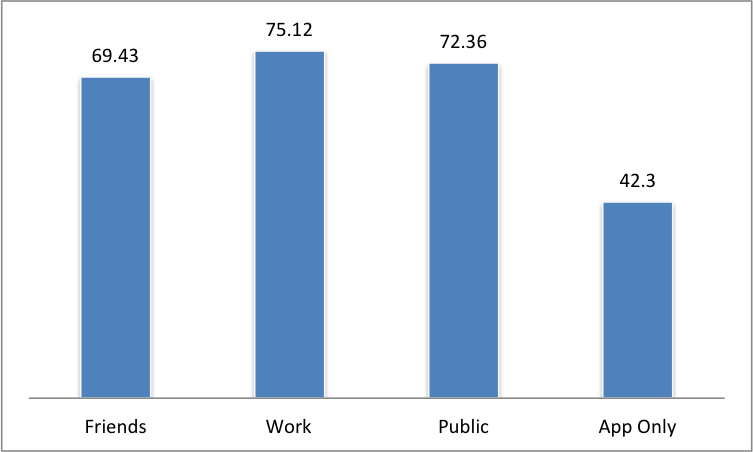
\includegraphics[width=0.5\textwidth]{recipient.png}
	\caption{(This is a placeholder! TODO: generate a better plot for data recipient)}
\end{figure}

\subsubsection{Device Type}


\begin{figure}
	\centering
	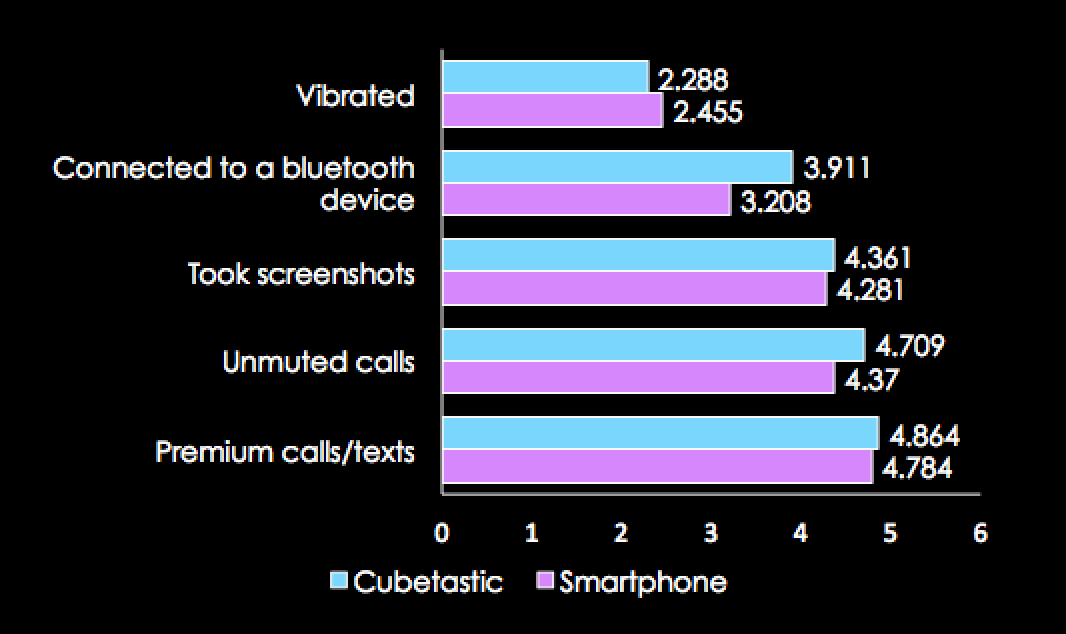
\includegraphics[width=0.5\textwidth]{device-type.png}
	\caption{(This is a placeholder! TODO: generate a better version of this)}
\end{figure}

\subsection{A Bigger Picture}

We asked users to rate how beneficial or risky a technology was, for all parties affected by the technology (including manufacturers, consumers, and bystanders), over a long period of time, with respect to other, well studied technologies. This gives us an interesting insight into how people perceive these new technologies. For instance, the capacity for facial detection on a wearable device is perceived to be as risky as interacting with a physical lawnmower. 

\begin{figure}
	\centering
	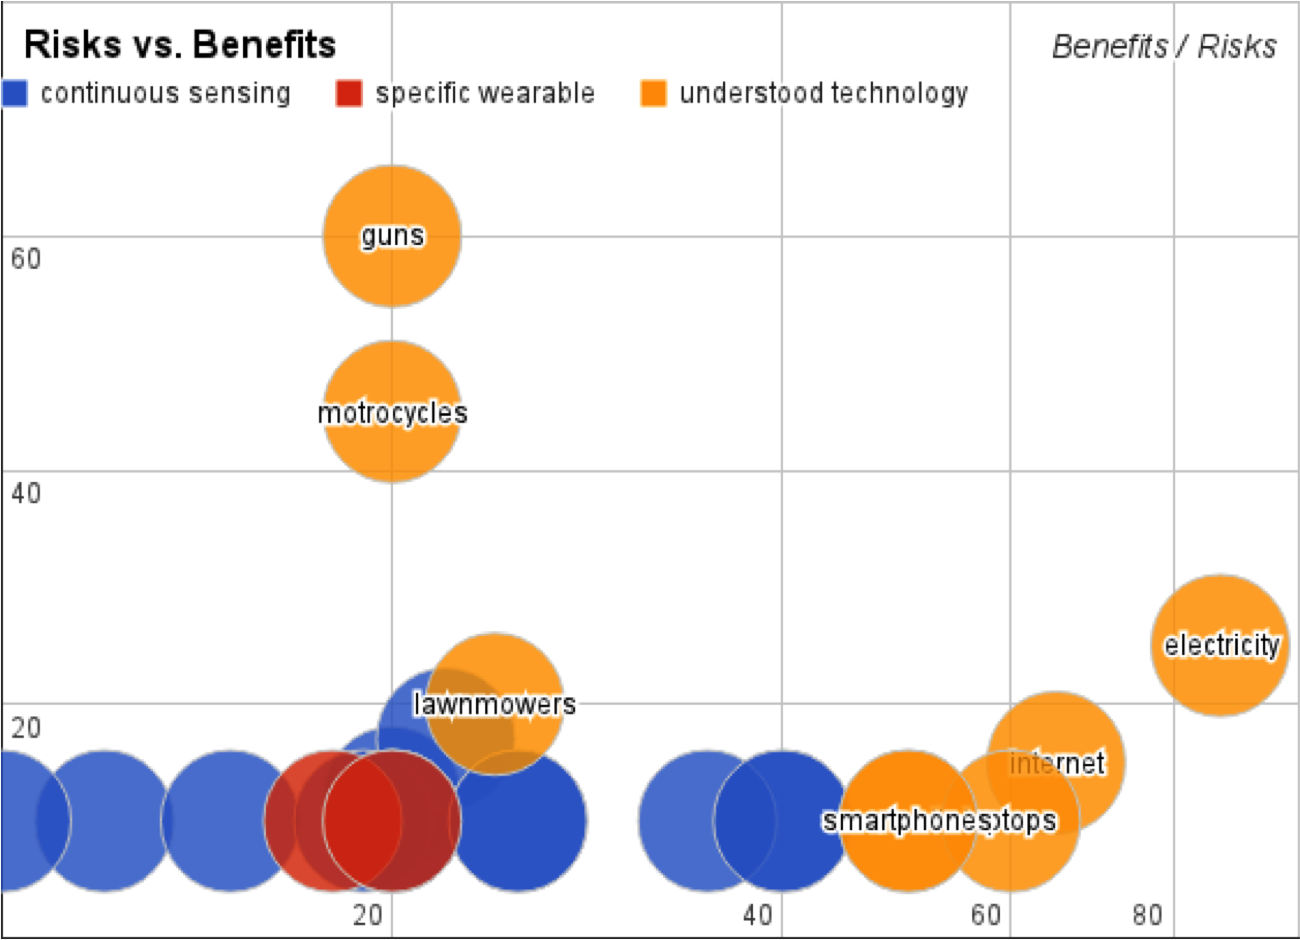
\includegraphics[width=0.5\textwidth]{techplot.png}
	\caption{(This is a placeholder! TODO: generate a better plot; take out the specific wearables too.)}
\end{figure}

\subsubsection{Risk and Benefit Ranks} 
\subsubsection{Lawnmower Ratios} 

\subsection{Perceived Concerns for Wearable Devices}

Although we asked users about particular situations which might occur with a wearable device and asked them to assess technologies in a general sense, our open ended question asked the users to state the most likely risk(s) associated with owning and interacting with wearable devices. Without any doubt, the most common concern for owning and interacting with wearable devices for the every day user is the \textit{loss of privacy}. 

Talk about the results of the open-ended answers here. 

%%%%%%%%%%%%%%%%%%%

\section{Discussion}
We take this section to discuss complementary future research directions in fields of privacy, ubiquitous computing, and user studies, along with specific limitations of this survey. 

\subsection{Future Research Directions}
(REDO, ask David's/Serge's input for this section) Additional future work is encouraged in the area of studying privacy with respect to ubiquitous computing, since we proved it was the number one concern of the users of wearable devices. Clearly, this is a hard question which has been worked on for a long time but not yet fully addressed. Even this survey just barely touched on the various factors which can influence privacy perceptions and how upset people would be. 

 Also, maybe some work with respect to security threats, and how feasible they might be, and some defenses against stopping wearables devices from getting sensitive information (like blocking text, detecting sensitive situations like the bathroom, etc.). Research which defends against false information, false positive commands, and just more safeguards against the new system for wearables, whatever that is, is also something to really look into. 
 
 Work making sure that people are aware of what is going on, using indicators, not-too-transparent interfaces, and maybe being polite (recording rules follow social rules--think polite glass talk from Jaeyeon at MSR) are going to be valuable as wearables get more sophisticated but also more adopted by people. Think about it--put people in control of the technology, not technology shifting the social norms (our survey says that one of the top concerns of people were about how wearables will change social norms). 

\subsection{Limitations}
One of the main limitations of this work is that our participants might not have interest, or an accurate idea, of wearable devices and their capabilities. 83\% of our participants reported that they do not own a wearable device, but at this time, about ~15\% of the general population own and use wearable devices \cite{Nilsen}\cite{WearableStatNews}, so our study is reflective of the status quo. We believed that getting a representative survey base was a useful endeavor, although we could have easily recruited only wearable device owners or people specifically interested in wearables. However, that will also have its own bias and limitations as well, since they would not reflect the general population. We expect user perceptions to change as rapidly as wearable technologies and the rate of adoption change. 

Crowdourcing user studies in Mechanical Turk has its challenges \cite{kittur2008crowdsourcing}. While the Amazon Mechanical Turk population is diverse across several significant demographic dimensions such as age, gender, and income, it is not a precise representation of the U.S. population \cite{ross2010crowdworkers}\cite{kelley2010conducting}. Additionally, Amazon Mechanical Turk workers generally put a higher value on anonymity and hiding information, were more likely to do so, had more privacy concerns than the larger U.S. public \cite{kang2014privacy}. 

The survey was constructed in a way to randomize the order of the particular sets of questions participants saw, except for the open-ended question, which was always near the end of the survey, asked along with the demographics. For this reason, people were heavily primed for the open-ended question. However, this question was always shown before the IUIPC questions, so our results on privacy being the top concern isn't because of the bias from the privacy index. The intent of the open-ended question  was more to get a sense of what people were concerned of, and we believe the results do reflect their actual concerns, but with a bit more clarity, since the participants were already thinking about such risks related to wearables. 

(REDO, Should I even say this?) I messed up that motorcycle question. I wish I actually had a calibration point for high risk high benefit for the Fischoff technology assessment questions. But well, none of the new technologies fit that description so we didn't really need it critically. 

%%%%%%%%%%%%%%%%%%%

\section{Conclusion}
END STRONG! Echo the conclusion a little, remind the people of the takeaways in a way that highlights the contribution of this paper. 


%\end{document}  % This is where a 'short' article might terminate

%ACKNOWLEDGMENTS are optional
\section{Acknowledgments}
NSF funding, SCRUB, BLUES. Also any people who helped.


%%%%%%%%%%%%%%%%%%%
%%%            BIB & ACKS          %%%
%%%%%%%%%%%%%%%%%%%

% The following two commands are all you need in the initial runs of your .tex file to produce the bib
%  and remember to run: latex bibtex latex latex to resolve all references

\bibliographystyle{abbrv}
\bibliography{wearables_survey}  % wearables_survey.bib is the name of the Bibliography


%APPENDICES are optional
%\balancecolumns
\appendix
%Appendix A
\section{Full Survey}
\section{Detailed Situation Rankings}
\section{Detailed Tech Rankings}
\section{Focus Group Script}

\balancecolumns

% That's all folks!
\end{document}
